\documentclass[12pt, titlepage]{article}

\usepackage{booktabs}
\usepackage{tabularx}
\usepackage{hyperref}
\usepackage{pdflscape}
\usepackage{graphicx}
\usepackage{amsmath}
\usepackage{float}
\hypersetup{
    colorlinks,
    citecolor=blue,
    filecolor=black,
    linkcolor=red,
    urlcolor=blue
}
\usepackage[round]{natbib}

%% Comments

\usepackage{color}

\newif\ifcomments\commentstrue %displays comments
%\newif\ifcomments\commentsfalse %so that comments do not display

\ifcomments
\newcommand{\authornote}[3]{\textcolor{#1}{[#3 ---#2]}}
\newcommand{\todo}[1]{\textcolor{red}{[TODO: #1]}}
\else
\newcommand{\authornote}[3]{}
\newcommand{\todo}[1]{}
\fi

\newcommand{\wss}[1]{\authornote{blue}{SS}{#1}} 
\newcommand{\plt}[1]{\authornote{magenta}{TPLT}{#1}} %For explanation of the template
\newcommand{\an}[1]{\authornote{cyan}{Author}{#1}}

%% Common Parts

\newcommand{\progname}{ProgName} % PUT YOUR PROGRAM NAME HERE
\newcommand{\authname}{Team \#, Team Name
\\ Student 1 name
\\ Student 2 name
\\ Student 3 name
\\ Student 4 name} % AUTHOR NAMES                  

\usepackage{hyperref}
    \hypersetup{colorlinks=true, linkcolor=blue, citecolor=blue, filecolor=blue,
                urlcolor=blue, unicode=false}
    \urlstyle{same}
                                


\begin{document}

\title{System Verification and Validation Plan for \progname{}} 
\author{\authname}
\date{\today}
	
\maketitle

\pagenumbering{roman}

\section*{Revision History}

\begin{tabularx}{\textwidth}{p{3cm}p{2cm}X}
\toprule {\bf Date} & {\bf Version} & {\bf Notes}\\
\midrule
2025-02-27 & 1.0 & Initial Release\\
\bottomrule
\end{tabularx}

\newpage

\tableofcontents
\listoftables

\listoffigures

\newpage
\section{Symbols, Abbreviations, and Acronyms}

\renewcommand{\arraystretch}{1.2}
\begin{tabular}{l l} 
  \toprule		
  \textbf{symbol} & \textbf{description}\\
  \midrule
  a & arbitrary positive integer\\
  CAS & Computing and Software\\
  CI & Continuous Integration\\
  CSV & Comma-Separated Values\\
  DE & Domain Expert \\
  $d_{total}$ & bin size, or number of binary descriptions \\
  $D_{bin}$ & 1D array of 32 byte binary strings \\
  FOV & field-of-view\\
  $I$ & 2D array of pixel values for a greyscale image \\
  $I'$ & transformed 2D array of pixel values\\
  $IFC$ & Image Feature Correspondences\\
  $k$ & number of total keypoints\\
  LD & Lead Developer \\
  $m$ & horizontal image dimension\\
  MG & Module Guide \\
  MIS & Module Interface Specification\\
  $n$ & vertical image dimension\\
  ORB & Oriented FAST and Rotated BRIEF\\
  $p$ & patch size\\
  PEP8 & Python Enhancement Proposal-8\\
  PNG & Portable Network Graphic\\
  PS & Project Supervisor\\
  RGB & Red-Green-Blue coloured imagery\\
  SDI & Software Design Instructor\\
  SLAM & Simultaneous Localization and Mapping\\
  SRS & Software Requirements Specification\\
  $t$ & intensity threshold \\
  VnV & Verification and Validation\\
  $\sigma$ & standard deviation\\
  \bottomrule
\end{tabular}\\

\newpage

\pagenumbering{arabic}
\noindent The intent of this document is to define the Verification and Validation (VnV) processes
that will be used to assess \progname, (IFC) software. Specifically, this document will be used to 
characterize the behaviour and performance of this software. The remaining sections of this document 
outline a detailed summary of the specific objectives of the VnV campaign. This includes considerations 
for the scope of the VnV efforts with respect to contraints that stem from the Winter 2025
development schedule, as well as anticipated activities for the Summer 2025 development cycle.
Verification procedures are present for select deliverables and milestone, and include 
an overview of anticipated cases for both system tests unit tests.

\section{General Information}

\subsection{Summary}
The Image Feature Correspondences (IFC) software is a feature comparison algorithm that is intended 
to be used as part of a pipeline to perform extrinsic camera calibration for 
applications in mobile robotics. It accepts camera configuration parameters and greyscale imagery data at 
different poses to identify common features amongst collected images. 

\subsection{Objectives}
The VnV process is intended to characterize how well the for the IFC software performs in its 
intended capacity to identify features amongst collected imagery. The performance of this system 
can vary significantly as it is influenced by factors such as overlap in camera fields-of-view (FOV),
the observed contrast between objects in an image, and variance in scale, rotation, and ambient 
illumination conditions. Furthermore, as there is no common baseline to compare this software to as 
an oracle, the VnV campaign for the IFC software is intended to characterize the performance of the 
integrated image processing functions against a set of test datasets. Key objectives of this process 
are defined below.

\begin{itemize}
  \item assess the reliability in the feature matching pipeline
  \item assess how users perceive their interactions with the IFC software 
  \item characterize the performances of the IFC software with metrics such as processing time and 
  memory usage
  \item cross-validate the performance of the IFC software with accepted benchmarked datasets
\end{itemize}
Verification of the individual functions within the OpenCV library themselves falls outside of the 
scope of this project, as we can assume that the library has been verified by its own 
implementation team. 
\\ \\

\subsection{Challenge Level and Extras}
% Updated to clearly indicate the challenge level of the project and how it consitutes the first portion of a larger image processing pipeline for MASc studies.
The proposed software constitutes a research project, as the IFC software serves as the front end of a robust optimization framework 
for extrinsic camera calibration. The IFC software must be capable of handling large volumes of high-resolution imagery while ensuring reliability through consistent and repeatable outputs. The software will be designed for robustness in data processing, accommodating a wide range of input conditions. Additionally, it will maintain a streamlined user experience, allowing users to override select default parameters while ensuring that the learning curve remains minimal for efficient adoption. 

As the long-term goal for this software is to absorb it into a larger calibration pipeline for research in the domain of mobile robotic, this project is defined as an advanced level of challenge. This program will supply a set of installation instructions, source code, test scripts, test imagery, and verification report. No additional documentation, such as a user manual will be provided.

\subsection{Relevant Documentation}
Relevant documentation has been hyperlinked throughout the length of the document. This enables 
the reader to access each resource within the context of the section that the reference is invoked.
\begin{itemize}
\item \textbf{Software Requirements Specification \href{https://github.com/KiranSingh15/CAS-741-Image-Correspondences/blob/main/docs/SRS/SRS.pdf}
{(SRS)}}
\item \textbf{Module Guide \href{https://github.com/KiranSingh15/CAS-741-Image-Correspondences/blob/main/docs/Design/SoftArchitecture/MG.pdf}
{(MG)}} 
\item 
\textbf{Module Interface Specification \href{https://github.com/KiranSingh15/CAS-741-Image-Correspondences/blob/main/docs/Design/SoftDetailedDes/MIS.pdf}{(MIS)}}
\end{itemize}

Additional document includes the checklists as follows.
\begin{itemize}
\item \textbf{\href{https://github.com/KiranSingh15/CAS-741-Image-Correspondences/blob/
main/docs/Checklists/SRS-Checklist.pdf}
{SRS Checklist}}. 
\item \textbf{\href{https://github.com/KiranSingh15/CAS-741-Image-Correspondences/blob/main/docs/Checklists/MG-Checklist.pdf}
{MG Checklist}} 
\item \textbf{\href{https://github.com/KiranSingh15/CAS-741-Image-Correspondences/blob/main/docs/Checklists/MIS-Checklist.pdf}{MIS Checklist}}
\item \textbf{\href{https://github.com/KiranSingh15/CAS-741-Image-Correspondences/blob/main/docs/Checklists/VnV-Checklist.pdf}
{VnV Checklist}}
\end{itemize}

\section{Plan}
This section outlines how each aspect of the VnV effort will be performed. This may be handled by 
milestone or by general practices, such as continuous integration and linters. 

\subsection{Verification and Validation Team}
The VnV team consists of four members, each of whom play a distinct role in the 
verification process. These roles and responsibilities are outlined in Table \ref{Table_Ver_Roles}.

\begin{table}[tbp!]
  \centering
  \begin{tabular}{|p{0.11\linewidth}|p{0.24\linewidth}|p{0.6\linewidth}|} 
    \hline
    \textbf{Name} & \textbf{Role} & \textbf{Description}\\
    \hline
    Kiran Singh & Lead Developer and Test Designer (LD) & Responsibilities include the
    identification of critical business cases for integrated tests, assessment of 
    schedule and scope considerations,  design and implementation of unit tests, 
    system tests, and documentation of test results.\\
    \hline
    Matthew Giamou & Project Supervisor (PS) & Lead consultant on integrated 
    performance needs and decomposition for software modules. Responsibilities 
    include review of proposed VnV scope, as proposed by 
    Kiran S., and provision of feedback to the general scope of the VnV campaign, and approval 
    of the individual test cases that are proposed by the LD. \\
    \hline
    Aliyah Jimoh & Domain Expert (DE) & Responsibilities include provision of 
    feedback on proposed test cases for the 
    scope of test cases for both the functional and non-functional requirements. They 
    will also provide feedback on the code walkthrough. 
    This statisfies the need for a reviewer that is removed from the design effort yet
    still holds sufficient domain knowledge to provide feedback on the overall design 
    and associated VnV efforts.\\ 
    \hline
    Spencer Smith & Software Development Instructor (SDI) & Responsibilities include 
    provision of feedback on proposed test cases for the scope of test cases 
    for both the functional and non-functional requirements. They will also 
    provide feedback via a code walkthrough. 
    This reviewer provides an essential stream of feedback as they are fully removed 
    from the application domain and may willing to question assumptions and address biases 
    that may be implicit amongst other members of the VnV team.\\
    \bottomrule
  \end{tabular}\\
  \caption{Roles and Responsibilities of the Verification and Validation Team}
  \label{Table_Ver_Roles}
\end{table}


\subsection{SRS Verification Plan}
The \textbf{\href{https://github.com/KiranSingh15/CAS-741-Image-Correspondences/blob/main/docs/SRS/SRS.pdf}
{SRS}} shall be reviewed by each member of the reviewer team to form consensus that the SRS has been correctly 
decomposed into sufficient requirements.
\begin{itemize}
\item the models are deemed to be comprehensible
\item the models are deemed to be correct
\item the associated requirements are traced correctly with respect to the models 
and project scope 
\item the requirements are decomposed in a manner that facilitates verification
\end{itemize}
Feedback on the \textbf{\href{https://github.com/KiranSingh15/CAS-741-Image-Correspondences/blob/main/docs/SRS/SRS.pdf}
{SRS}}
 from the DE and SDI will be captured through 
the use of Github Issues. Specifically, both reviewers will use the 
\textbf{\href{https://github.com/KiranSingh15/CAS-741-Image-Correspondences/blob/
main/docs/Checklists/SRS-Checklist.pdf}
{SRS Checklist}}. 
The lead developer will respond in turn to each issue and if 
reserves the right to reject a proposed change as needed. \\
The Lead Developer will schedule a meeting with the Project Supervisor to walk through 
the first revision of the \textbf{\href{https://github.com/KiranSingh15/CAS-741-Image-Correspondences/blob/main/docs/SRS/SRS.pdf}
{SRS}}
 document. In this meeting, the Project Supervisor will offer 
feedback and recommendations for candidate revisions to the outlined models and requirements. 
The Lead Developer will then create issues in Github to address each proposed revision.

\subsection{Design Verification Plan}
The DE and SDI will review the Module Guide 
\textbf{\href{https://github.com/KiranSingh15/CAS-741-Image-Correspondences/blob/main/docs/Design/SoftArchitecture/MG.pdf}
{(MG)}} and the Module Interface Specification 
\textbf{\href{https://github.com/KiranSingh15/CAS-741-Image-Correspondences/blob/main/docs/Design/SoftDetailedDes/MIS.pdf}
{(MIS)}} against the 
\textbf{\href{https://github.com/KiranSingh15/CAS-741-Image-Correspondences/blob/main/docs/Checklists/MG-Checklist.pdf}
{MG Checklist}} and
\textbf{\href{https://github.com/KiranSingh15/CAS-741-Image-Correspondences/blob/main/docs/Checklists/MIS-Checklist.pdf}
{ Checklist}}. The objective of this review cycle is to ensure that the design of the system:
\begin{enumerate}
\item is unambiguous
\item adheres to best-practices of module design
\item aligns with the requirements as identified in the 
\textbf{\href{https://github.com/KiranSingh15/CAS-741-Image-Correspondences/blob/main/docs/SRS/SRS.pdf}
{SRS}}
\end{enumerate}


\subsection{Verification and Validation Plan Verification Plan}
The VnV Plan will be verified via inspection by the DE and the 
Software Development Instructor. The 
\textbf{\href{https://github.com/KiranSingh15/CAS-741-Image-Correspondences/blob/main/docs/Checklists/VnV-Checklist.pdf}
{VnV Plan Checklist}} 
will be used as the assessment criteria for the inspection. 
Feedback will provided as Github issues and will be handled in the same manner as feedback 
for the SRS.\\ \\

% Removed discussion of mutation testing due to schedule constraints.

\subsection{Implementation Verification Plan}
% updateed to remove reference to CAS 741 per Issue #9
The IFC software shall be verified against the test procedures outlined in Sections \ref{FR_Tests} and 
\ref{NFR_Tests}. Static verification of the IFC software will consist of a code walkthrough. This will take 
place on April 4th, 2025, during which the the DE and SDI will have the opportunity to observe 
the code and raise issues following the presentation via GitHub. \\ \\
Dynamic verification of the IFC software will consist of system and unit tests via PyTest. System tests 
are outlined in Section \ref{Sys_Tests}. Unit tests will be outlined in Rev 2 of the VnV Plan in 
Section \ref{UTD}.

\subsection{Automated Testing and Verification Tools}
Several tools will be used to support automated testing and verification. They include:
\begin{itemize}
\item Continuous Integration (CI) will be facilitated via GitHub Actions. A pull request will be used 
to run automated tests.
\item Pytest will be used to execute system tests, unit tests, and to assess code coverage. 
\item flake8 will be used as a linter to ensure adherence to PEP8 standards. 
% Pylint has been removed in favour of flake8
\end{itemize}

\subsection{Software Validation Plan}
% Updated per Instructor feedback on Rev 1.0
Validation testing has been identified as out of scope for the IFCS software.

\section{System Tests}\label{Sys_Tests}
This section outlines the general roadmap for the required integrated system tests. 
\subsection{Tests for Functional Requirements} \label{FR_Tests}
This section outlines the system tests that verify the requirements outlined in 
Section 5 of the 
\textbf{\href{https://github.com/KiranSingh15/CAS-741-Image-Correspondences/blob/main/docs/SRS/SRS.pdf}
{SRS}}. 

\begin{figure}[h!]
  \begin{center}
   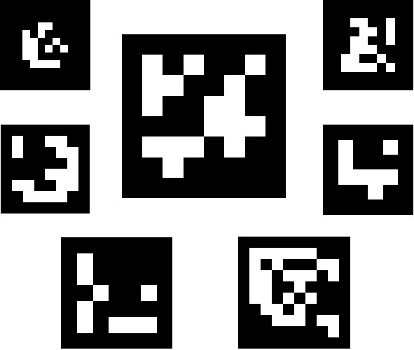
\includegraphics[width=0.6\textwidth]{images/ArUco_Field_Gen.jpg}
  \caption[An example of a generated ArUco pattern]{An example of a generated ArUco pattern. Image taken 
  from \cite{ARUCO_Markers_openCV}}
  \label{gen_aruco} 
  \end{center}
\end{figure}

\begin{figure}[h!]
  \begin{center}
   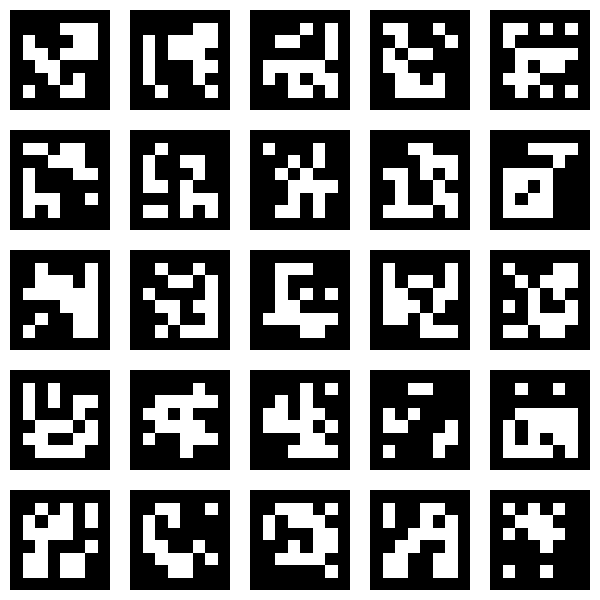
\includegraphics[width=0.6\textwidth]{images/aruco_000.png}
  \caption[An example of ArUco patterns within the scene of a captured greyscale image]
  {Expected baseline ArUco pattern for functional tests STFR-IS-01, STFR-KP-01, STFR-FD-01, and STFR-FM-01}
  \label{gs_aruco_field} 
  \end{center}
\end{figure}

\subsubsection{Feature Detection}
This test section is intended to assess that the system can accept new parameters from users and covers 
requirements R1 through R7 and R9 through R11, in Section 5.1 of the 
\textbf{\href{https://github.com/KiranSingh15/CAS-741-Image-Correspondences/blob/main/docs/SRS/SRS.pdf}
{SRS}}. 
		
\paragraph{Image Smoother}
\begin{enumerate}
\item \hypertarget{STFR-IS-01}{\textbf{STFR-IS-01}}

\textbf{Requirements Addressed:} R1, R5, R9

\textbf{Control:} Automated		

\textbf{Initial State:} Uninitialized

\textbf{Input:} Generated binary patterned fiducial markers, named 
\href{https://docs.opencv.org/4.x/d5/dae/tutorial_aruco_detection.html}
{ArUco} markers, will be used as simplified targets for corner detection. The script that is used to generate these images is provided in the src code, \href{https://github.com/KiranSingh15/CAS-741-Image-Correspondences/blob/main/src/tests/gen_arcuo.py}{gen\_aruco.py}.A depiction of these markers is shown in Figure \ref{gen_aruco}. This script generates an initial image with contains 25 $6\times 6$-bit ArUco markers. It uses a seed of 42 to perform scaling, rotational, and translational transforms on the baseline marker. These transforms range between $-45^\circ$ and $45^\circ$, 30 pixels of lateral translation, and a scaling factor between 0.5 and 0.9. A total of 20 transformed images are produced as inputs for the test. Each image $I$ is defined as a 2D image of $600 \times 600$ pixel resolution. A Gaussian smoothing kernel of 5 and standard deviation of 1.0 will be used to smooth the edges of the imagery. 

\textbf{Output:} 20 output images as a 2D array, each of which have a descriptive name that clearly identifies the input image from which it originates. In this case, all images should use the convention of 'aruco\_xxx.png', where 'xxx' represents the enumerated ID of the ArUco marker. The output image, $I'$, should be of equal size and the same data type as its 
corresponding image $I$. All images should be saved under a distinct folder to prevent mixing of input and output imagery.

\textbf{How test will be performed:} Automated Tools (i.e. Pytest). If the ArUco imagery is not provided in the src/tests folder, then the user needs to run the gen\_aruco.py script to generate the test imagery. Once complete, the user needs to only run STFR-IS-01.py via Pytest while in the src folder to run the test. The pytest file then checks each generated image to confirm that it has the same size and image datatype as the original input image. If each image has a resolution of $600 \times 600$ pixels and is an image of type unit8, then the test is considered a pass.

\end{enumerate}


\paragraph{Keypoint Detector}
\begin{enumerate}
\item \hypertarget{STFR-KP-01}{\textbf{STFR-KP-01}\\}
\textbf{Requirements Addressed:} R2, R6, R10

\textbf{Control:} Automatic	

\textbf{Initial State:} Uninitialized			

\textbf{Input:} A collection of 20 smoothed PNG images $I'$ with a resolution of $600\times 600$ that 
contain the same ArUco markers as outlined in System Test \hyperlink{STFR-IS-01}{STFR-IS-01}. The user assigns a pixel intensity threshold ($t$) of 60.

\textbf{Output:} A flag which indicates that corner detection is active. 
A 2D array of size ${k \times m}$, where $k$ is the quantity of identified keypoints and the first and second columns are populated with the horizontal and vertical coordinates for each keypoint. Each entry in the array should be rounded to a positive integer value. Any outstanding columns may be populated with associated metadata as a product of the selected method of keypoint detection. For example, oriented FAST (o-FAST) differs from standard FAST in that it also provides an measure of rotation for each keypoint as an additional column. Each array should have a unique title that clearly defines the original image from which its keypoints were identified. All output arrays should be saved to a unique folder to separate them from the input images.

\textbf{How test will be performed:} Automated Tools (i.e. Pytest)If the smoothed ArUco imagery is not provided in the src/tests folder, then the user needs to run the gen\_aruco.py script to generate the test imagery. Once complete, the user needs to only run STFR-KP-01.py via Pytest while in the src folder to run the test. The Pytest file then checks each row of the generated CSV file to confirm that each x and y coordinate is rounded to an integer value. If any keypoint does not contain either an x or y coordinate, a flag is raised and is reported. If all x and y coordinates are rounded to the nearest integer, then the test is deemed to be a pass.
\end{enumerate}

\paragraph{Feature Definition}
\begin{enumerate}
\item \hypertarget{STFR-FD-01}{\textbf{STFR-FD-01}\\}
\textbf{Requirements Addressed:} R3, R4, R7, R11

\textbf{Control:} Automatic

\textbf{Initial State:} Uninitialized

\textbf{Input:} A collection of 20 PNG images with a resolution of $600\times 600$, where each image features 25 $6\times 6$ ArUco markers within the scene. A $k\times m$ 2D array will be provided for each image, where $k$ is the number of keypoints within each image. A target bin size ($d_{total}$) of 100 will be used to define the target number of feature descriptors. A patch size ($p$) of 31 will be used to define the adjacent region of a keypoint for which to define descriptors.

\textbf{Output:} $D_{bin}$, an array of length $d_{total}$ with a minimum width of 1 where all entries of the array are 32 byte binary strings. The width of this array may be increased if associated horizontal and vertical coordinates for the corresponding keypoint may be affixed to each descriptor. 

\textbf{Test Case Derivation:} \href{https://sites.cc.gatech.edu/classes/AY2024/cs4475_summer/images/ORB_an_efficient_alternative_to_SIFT_or_SURF.pdf}
{ORB: An efficient alternative to SIFT or SURF}. This publication outlines methods to develop and the corresponding assessment of binary feature descriptors.

\textbf{How test will be performed:} Automated Tools (i.e. Pytest). If the smoothed ArUco imagery is not provided in the src/tests folder, then the user needs to run the gen\_aruco.py script to generate the test imagery. Once complete, the user needs to only run test\_STFR-FD-01.py via Pytest while in the src folder to run the test. The Pytest file then checks each row of the generated CSV file to confirm that each descriptor has a horizontal and vertical coordinate, rounded to the nearest integer. All 256 bits of the binary descriptor are then checked to ensure that there is no data bit loss from conversion to CSV. If associated horizontal or vertical coordinates are identified as missing, then the test fails. If there is any loss of databit within the 32 byte descriptor, then the test fails. If all identified descriptors pass both the coordinates and descriptor bitwise checks, then the test is defined to be a pass.
\end{enumerate}

\subsubsection{Feature Comparison}

This test section is intended to assess that the system can accept new parameters from users. It addresses 
requirements R8 and R12 through R15 in Section 5.1 of the 
\textbf{\href{https://github.com/KiranSingh15/CAS-741-Image-Correspondences/blob/main/docs/SRS/SRS.pdf}
{SRS}}. 
		
\paragraph{Descriptor Comparison}
\begin{enumerate}
\item \hypertarget{STFR-FM-01}{\textbf{STFR-FM-01}\\}
\textbf{Requirements Addressed:} R8, R12, R13, R14, R15

\textbf{Control:} Automated		

\textbf{Initial State:} Uninitialized

\textbf{Input:} 20 1D arrays, each which have a unique length, $D_{bin}$, where each element of the 
array is a 32 byte binary string known as a binary descriptor. Each array should be labeled with a 
descriptive name that clearly references the instance of both the camera and pose at the time of image 
capture.

\textbf{Output:} A flag that indicates that Hamming Distances were compared. A dynamically-sized array, stored as a Pandas dataframe, where the length of the array is the number of matched features. The columns of the array will include the properties as follows.
\begin{itemize}
\item Binary descriptors of both features as 32 byte binary strings
\item Corresponding image IDs for each feature
\item Matching scores between both features
\item The Hamming Distance of each candidate match between features
\end{itemize}
% Introduced to address the question of "What is the Correct Hamming Distance?" per feedback on Rev 1.0
Note that we do not compare the identified Hamming Distance as there is no baseline Hamming Distance for which to compare. \\

\textbf{How test will be performed:} Automated Tools (i.e. Pytest)
If the smoothed ArUco imagery is not provided in the src/tests folder, then the user needs to run the gen\_aruco.py script to generate the test imagery. Once complete, the user needs to only run test\_STFR-FM-01.py via Pytest while in the src folder to run the test. The Pytest file then checks each row of the generated CSV file to confirm that for both pairs of descriptors that compose a candidate match, each descriptor has a horizontal and vertical coordinate, rounded to the nearest integer. All 256 bits of the binary descriptor are then checked to ensure that there is no data bit loss from conversion to CSV. Finally, the calculated distance between each descriptor is assessed to confirm that it is a positive integer. If associated horizontal or vertical coordinates are identified as missing, then the test fails. If there is any loss of databit within the 32 byte descriptor, then the test fails. If the distance between descriptors is not a positive integer, the test fails. If all identified descriptors pass both the coordinates and descriptor bitwise checks, and the distance is a positive integer, then the test is defined to be a pass.
\end{enumerate}

\subsection{Tests for Nonfunctional Requirements}\label{NFR_Tests}
\subsubsection{Reliability}
The IFC software is envisioned to be used as part of the front end of a larger camera calibration pipeline, 
where the outputs of the IFC software need to produce consistent results for use in a back-end optimization 
module. Therefore, the IFC software needs to undergo verification to ensure that it can match the same 
features between two images. The following system test satisfies \textbf{NFR1} of the 
\textbf{\href{https://github.com/KiranSingh15/CAS-741-Image-Correspondences/blob/main/docs/SRS/SRS.pdf}
{SRS}}.

\paragraph{Repeatability}
\begin{enumerate}
\item \hypertarget{STNFR-RE-1}{\textbf{STNFR-RE-1}\\}
\textbf{Type: Dynamic}

\textbf{Initial State:} Uninitialized

\textbf{Input/Condition:} Two datasets of imagery data. These datasets contain the same collection of images, 
but are arranged in a different order.

\textbf{Output/Result:} The feature matching pipeline will be use to identify features and compare them amongst 
images for both datasets. For both datasets, a dynamically-sized array will be output. These arrays will 
contain the feature descriptors and the image IDs of origin, as specified in as specified in 
\hyperlink{STFR-DC-01}{STFR-DC-01}. 
One array will be reordered to reflect the order of the other array. Once the second array has been reordered, 
the arrays will be compared in terms of their length and contents. For example, in images A and B, they will be 
processed under the pseudonym of B' and A', respectively. That is, for each feature of A, its descriptor and x-y 
coordinates are equivalent to those of B'. Similarly, the coordinates and descriptor of B are equivalent to A'. 
The features of A and B will be compared to identify matches. Then the features of A' and B' will be compared as 
well. The test will be considered a pass if the identified matches between A and B share the same descriptors and 
coordinates as the identified matches between B' and A', respectively.

\textbf{How test will be performed:} PyTest. Two sample images from the Lego library have been duplicated and reordered with new names. Paths to the original and transformed images are outlined in the  test\_STFR-RE-01.py file. A script will assess that for the corresponding transformed image, that the same coordinates and 32-byte feature descriptor are identified as a match candidate with the same coordinates and 32-byte descriptor of the transformed image for the complementary image.
\end{enumerate}

\subsubsection{Usability}
As part of a larger pipeline, the IFC software needs to be simple for its users to integrate into the calibration system. 
This may be reflected in the perception of how simple it is for the user to 
implement its on their own system and to run the program as its own module. This usability criterion is 
reflected in \textbf{NFR2} of the 
\textbf{\href{https://github.com/KiranSingh15/CAS-741-Image-Correspondences/blob/main/docs/SRS/SRS.pdf}
{SRS}}.

\paragraph{User Experience: End-to-End Feature Matching}
\begin{enumerate}
\item \hypertarget{STNFR-UX-1}{\textbf{STNFR-UX-1}\\}
\textbf{Type:} Dynamic

\textbf{Initial State:} Uninitialized

\textbf{Output/Result:} A dataframe of identified features, as outlined in \hyperlink{STFR-DC-01}{STFR-DC-01}. 
Once the test has been completed, the user will be asked to express their opinion of their experience of the 
system, and to remark on the following topics.
\begin{itemize}
\item the degree of perceived difficulty in preparing the input files
\item the degree of perceived difficulty in assignment of the camera properties
\item the user's overall satisfaction with using the program
\end{itemize} 

\textbf{How test will be performed:} Dynamic Test by User
\end{enumerate}
The characteristics of the desired user are outlined in the \textbf{\href{https://github.com/KiranSingh15/CAS-741-Image-Correspondences/blob/main/docs/SRS/SRS.pdf}{SRS}}. However, for the intent of testing, the user may be defined as the Project Supervisor or Domain Expert. The user will be provided a collection of images from different cameras. Each image will be labelled with 
a descriptive title that clearly defines what camera the image originates from. The user shall be responsible 
to insert all images into a common folder.

The user shall execute the following procedure in the following order.
\begin{enumerate}
  \item The user shall open the directory to the IFC configuration file.
  \item In the IFC program configuration file, the user shall:
  \begin{enumerate}
      \item Update the input location as the folder of all the input images.
      \item Update the system directory with the desired location of the matched feature array.
      \item Assign a directory for altered imagery, if desired.
      \item Input the number of cameras per the sized camera data.
      \item Provide the following details for each camera:
      \begin{enumerate}
          \item A descriptive name of the camera that matches the prefix of the name of its imagery data.
          \item The resolution of each camera.
      \end{enumerate}
  \end{enumerate}
  \item The user shall close the IFC configuration file.
  \item The user initiates execution of the feature comparison pipeline.
  \item The user waits for the image comparison process to complete.
  \item After completion, the user opens the output array directory.
  \item The user reviews the output array to verify that there are no errant characters.
  \item The user closes the output array.
\end{enumerate}
\mbox{} \\
Though not within the current scope of the VnV plan, a separate test may be performed where the 
user performs the same steps as \hyperlink{STNFR-UX-1}{STNFR-UX-1}, 
and additionally modifies the Gaussian Kernel standard distribution, intensity threshold, and patch size 
parameters to values within the allowable operational boundaries. 


\subsubsection{Maintainability}\label{Maintainability}
Verification of \textbf{NFR3}, outlined in 
\textbf{\href{https://github.com/KiranSingh15/CAS-741-Image-Correspondences/blob/main/docs/SRS/SRS.pdf}
{SRS}}, 
has been delegated as future work in favour of other verification procedures outlined within this 
document. This tradeoff was made to satisfy the schedule and developer resource constraints of the Winter 2025 development cycle. 
It would however, be simple to evaluate if a new detection was to be implement. Once the default feature 
detection method has successfully been completed, the total number of hours spent to design the feature 
detection module should be summed together. A factor of 0.3 should be applied to the summed effort to define 
the maximum target effort to develop a new method of feature detection. Any time that is dedicated to 
implement a new method should be added to the running total. A scenario where the total effort exceeds the 
allowable target may suggest that the current IFC software is difficult to maintain.

\subsubsection{Performance}\label{Performance}
One of the primary objectives of the VnV campaign is to characterize what system resources are required to 
execute the IFC software, as outline in \textbf{NFR4} and \textbf{NFR5}. In the case of a simple configuration 
with only two cameras at two different poses, the process is trivial. However, for configurations that consist 
of as many as ten cameras across dozens of robot poses, the problem may scale significantly. Therefore, as a 
general practice, timing and memory usage metrics should be recorded throughout the duration of any of the 
primary operations of the IFC software. This includes the following system tests in Section \ref{FR_Tests}. 
\begin{enumerate}
\item \hyperlink{STFR-IS-01}{STFR-IS-01}
\item \hyperlink{STFR-KP-01}{STFR-KP-01}
\item \hyperlink{STFR-FD-01}{STFR-FD-01}
\item \hyperlink{STFR-DC-01}{STFR-DC-01}
\end{enumerate}
\paragraph{Timing Metrics}
\mbox{}
\\
The timestamp will be recorded at the start of each of the major operations (i.e. 
Image Smoothing, Keypoint Detection, Assignment of Feature Descriptors, and Feature Comparison). 
A subsequent timestamp will be recorded after the termination of each operation. The difference between 
the start and termination timestamps will be saved and stored in a structured format 
(e.g., JSON or CSV) within a designated log directory.

\paragraph{Memory Usage Metrics}
\mbox{}
\\
The memory usage of the IFC software should be logged with a timestamp and operation identifier and stored 
in a structured format (e.g., JSON or CSV) within a designated log directory. This data may also be augmented 
with a separate file that outlines the average memory usage, and the peak memory usage with associated 
timestamps.



\newpage
\subsection{Traceability Between Test Cases and Requirements}
The traceability between each scoped test case and its respective requirements is outlined by 
\ref{Table_R_trace}.

\begin{table}[h!]
  \centering
  \begin{tabularx}{\textwidth}{|c|X|X|X|X|X|X|}
  \hline
  \textbf{}     & \textbf{STFR-IS-01} & \textbf{STFR-KP-01} & \textbf{STFR-FD-01} & \textbf{STFR-FM-01} & \textbf{STNFR-RE-1} & \textbf{STNFR-UX-1} \\ \hline
  \textbf{R1}   & x                   &                     &                     &                     &                     &                     \\ \hline
  \textbf{R2}   &                     & x                   &                     &                     &                     &                     \\ \hline
  \textbf{R3}   &                     &                     & x                   &                     &                     &                     \\ \hline
  \textbf{R4}   &                     &                     & x                   &                     &                     &                     \\ \hline
  \textbf{R5}   & x                   &                     &                     &                     &                     &                     \\ \hline
  \textbf{R6}   &                     & x                   &                     &                     &                     &                     \\ \hline
  \textbf{R7}   &                     &                     & x                   &                     &                     &                     \\ \hline
  \textbf{R8}   &                     &                     &                     & x                   &                     &                     \\ \hline
  \textbf{R9}   & x                   &                     &                     &                     &                     &                     \\ \hline
  \textbf{R10}  &                     & x                   &                     &                     &                     &                     \\ \hline
  \textbf{R11}  &                     &                     & x                   &                     &                     &                     \\ \hline
  \textbf{R12}  &                     &                     &                     & x                   &                     &                     \\ \hline
  \textbf{R13}  &                     &                     &                     & x                   &                     &                     \\ \hline
  \textbf{R14}  &                     &                     &                     & x                   &                     &                     \\ \hline
  \textbf{R15}  &                     &                     &                     & x                   &                     &                     \\ \hline
  \textbf{NFR1} &                     &                     &                     &                     & x                   &                     \\ \hline
  \textbf{NFR2} &                     &                     &                     &                     &                     & x                   \\ \hline
  \textbf{NFR3*}& -                    & -                   & -                   & -                   & -                   & -                   \\ \hline
  \textbf{NFR4} & o                   & o                   & o                   & o                   &                     &                     \\ \hline
  \textbf{NFR5} & o                   & o                   & o                   & o                   &                     &                     \\ \hline
  \end{tabularx}
  \caption{Traceability Matrix Showing the Connections Between Requirements and Instance Models}
  \label{Table_R_trace}
\end{table}

\begin{itemize}
\item \lq x\rq{} indicates a direct method of verification
\item \lq o\rq{} indicates an indirect method of verification
\item * Verification of NFR3 is defined as outside of scope per Section \ref{Maintainability}
\end{itemize}


\section{Unit Test Description}\label{UTD}
This section describes the unit tests developed for the Image Feature Correspondences (IFC) system. The tests validate that the system conforms to the functional and nonfunctional requirements specified in the SRS and implemented per the design in MIS. The unit tests are executed using the \texttt{pytest} framework and primarily assess correctness, parameter bounds, default behavior, and file outputs.

The test strategy includes both black-box and white-box testing:
\begin{itemize}
  \item \textbf{Black-box testing} ensures that each module produces expected results given a specific input.
  \item \textbf{White-box testing} checks internal method logic, parameter validation, and error handling.
\end{itemize}

All modules have unit tests verifying both normal and edge case behavior. Each test function name corresponds to its functionality and is self-documenting.

\subsection{Unit Testing Scope}

Testing of the OpenCV Module itself is considered out of scope.

\subsection{Tests for Functional Requirements}
Note that the unit tests are not outlined in the numerical order of the modules (i.e. M1, M2, etc.) as it is intended to reflect a gradual increase in complexity of unit testing up to the \textbf{Control Module (M2)}. A full breakdown of the unit tests can be found in the \href{https://github.com/KiranSingh15/CAS-741-Image-Correspondences/tree/main/test}{\textbf{test}} folder of the Github Repository.


\subsubsection{Module: Specification Parameters Module (M4)}
This module is responsible for housing the script that enables the users to configure the methods of image processing will be used in the pipeline and to adjust the respective tuning parameters for each method.

\begin{enumerate}
  \item \texttt{test\_kernel\_bounds} \textnormal{(from \texttt{test\_specParams.py})}. \\

  Type: Unit, Automatic

  Initial State: A predefined kernel value \texttt{test\_k} and kernel bounds \texttt{lim\_kern\_bounds = [3, 15]}.

  Input: An integer representing a Gaussian kernel size.

  Output: Assertion pass/fail depending on whether the kernel size is odd and within the inclusive bounds.

  Test Case Derivation: This test is a simple check to ensure that the select kernel size is compatible with Gaussian filtering operations.

  How test will be performed: Implemented via automated Pytest script and Github Actions. Checks that \texttt{test\_k} is of type \texttt{int}, odd-valued, and lies within the bounds.

  \item \texttt{test\_standard\_deviation} \textnormal{(from \texttt{test\_specParams.py})}. \\

  Type: Unit, Automatic

  Initial State: A defined standard deviation value \texttt{test\_sigma} and limits \texttt{lim\_sd\_bounds = (0, 10]}.

  Input: A float or integer representing Gaussian standard deviation.

  Output: Assertion pass/fail if the value is not in \((0, 10]\), accounting for floating-point precision.

  Test Case Derivation: Supports \textbf{R01}, validating continuous parameter constraints for Gaussian blur.

  How test will be performed: Automated script via Pytest and GitHub Actions. Type-checked and validated using an epsilon margin for numerical stability.

  \item \texttt{test\_fast\_bounds} \textnormal{(from \texttt{test\_specParams.py})}. \\

  Type: Unit, Automatic

  Initial State: FAST detection threshold \texttt{test\_t} and intensity limits \texttt{lim\_fast\_bounds = [2, 254]}.

  Input: An integer intensity threshold value.

  Output: Boolean result from assertion checking bounds compliance.

  Test Case Derivation: Supports \textbf{R02}, ensuring intensity threshold parameterization for corner detection.

  How test will be performed: Automated script via Pytest and GitHub Actions. The test asserts that the value lies within bounds and is an integer.

  \item \texttt{test\_bin\_bounds} \textnormal{(from \texttt{test\_specParams.py})}. \\

  Type: Unit, Automatic

  Initial State: Descriptor bin count \texttt{test\_b}, constrained by \texttt{lim\_bin\_bounds = [1, 2048]}.

  Input: Integer representing number of ORB descriptors to retain.

  Output: Passes if within bounds, otherwise assertion error is raised.

  Test Case Derivation: Enforces \textbf{R04}, which governs descriptor configuration consistency.

  How test will be performed: Automated script via Pytest and Github Actions. Type and range checks performed on the bin size.

  \item \texttt{test\_patch\_size\_bounds} \textnormal{(from \texttt{test\_specParams.py})}. \\

  Type: Unit, Automatic

  Initial State: Descriptor patch size \texttt{test\_p} bounded by \texttt{lim\_patch\_sz = [5, 100]}.

  Input: Integer specifying the spatial extent for descriptor extraction.

  Output: Assertion checks for compliance with defined patch size range.

  Test Case Derivation: Related to \textbf{R03}, controlling spatial descriptor characteristics.

  How test will be performed: Automated script via Pytest and Github Actions. The patch size is verified to be an integer and within range.

  \item \texttt{test\_avail\_methods} \textnormal{(from \texttt{test\_specParams.py})}. \\

  Type: Unit, Automatic

  Initial State: Lists of available methods defined in \texttt{SpecificationParametersModule.py}:
  \texttt{mthd\_is}, \texttt{mthd\_kpd}, \texttt{mthd\_fd}, \texttt{mthd\_ftm}.

  Input: None (test inspects module-level variables).

  Output: Assertion passes if each method list is a non-empty list or tuple.

  Test Case Derivation: Supports \textbf{R06}, \textbf{R07}, and \textbf{R08} to ensure at least one method is implemented for each stage of the pipeline.

  Test Cases:
  \begin{itemize}
    \item All lists are non-empty and of valid types (expected outcome: pass)
    \item \texttt{mthd\_is = []} (expected outcome: fail)
    \item \texttt{mthd\_fd = "ORB"} (expected outcome: fail)
  \end{itemize}

  How test will be performed: Automated script via Pytest and GitHub Actions. Module is imported and assertions are applied directly to global method lists without requiring user input.

  \item \texttt{test\_selected\_methods} \textnormal{(from \texttt{test\_specParams.py})}. \\

  Type: Unit, Automatic

  Initial State: User-selected method identifiers from \texttt{SpecificationParametersModule.py}:
  \texttt{mthd\_img\_smoothing}, \texttt{mthd\_kp\_detection}, \texttt{mthd\_kp\_description}, \texttt{mthd\_ft\_match}.

  Input: Enumerated integer selections for each image processing stage.

  Output: Assertion passes if all values are integers and \(\geq 0\).

  Test Case Derivation: Automated script via Pytest and GitHub Actions. Supports ,\textbf{R06, R07, R08}, ensuring valid configuration and preventing undefined method selection.

  Test Cases:
  \begin{itemize}
    \item All values are valid integers \(\geq 0\) (e.g., 1, 2, 3; expected outcome: pass)
    \item \texttt{mthd\_img\_smoothing = -1} (expected outcome: fail)
    \item \texttt{mthd\_ft\_match = "brute\_force"} (expected outcome: fail)
  \end{itemize}

  How test will be performed: Automated script via Pytest and GitHub Actions. Module-level configuration parameters are evaluated and asserted for type and range correctness.
\end{enumerate}



\subsubsection{Module: Input Format Module (M3)}

This module is responsible for validating user inputs, setting defaults, and enforcing parameter bounds.

\begin{enumerate}
\item{test\_check\_parameter\_limits\_valid\\}

Type: Functional, Automatic
          
Initial State: All parameters, including standard deviation $\sigma$ = 1.5, are within valid bounds.

Input: $\sigma = 1.5$

Output: No assertion error; standard deviation value accepted.

Test Case Derivation: Satisfies \textbf{R01} where user input for $\sigma$  falls within allowable range $(0, 10]$.

How test will be performed: Automated via Pytest and GitHub Actions using parameterized validation checks in \texttt{check\_parameter\_limits()}.

\item{test\_check\_parameter\_limits\_valid\\}

Type: Functional, Automatic

Initial State: Threshold t = 100

Input: t = 100

Output: No assertion error; threshold value accepted.

Test Case Derivation: Address \textbf{R02} where the user-defined input for FAST threshold lies within [2, 254].

How test will be performed: Automated via Pytest and GitHub Actions using valid parameter combination.

\item{test\_check\_parameter\_limits\_valid\\}

Type: Functional, Automatic

Initial State: Patch size = 20

Input: Patch size = 20

Output: No assertion error; patch size is accepted.

Test Case Derivation: Addresses \textbf{R03} to confirm that patch size lies within range [5, 100] and is integer.

How test will be performed: Automated script via Pytest and GitHub Actions using structured parameter validation.

\item{test\_check\_parameter\_limits\_valid\\}

Type: Functional, Automatic

Initial State: Bin size = 128

Input: bin size = 128

Output: No assertion error; bin size accepted.

Test Case Derivation: Addresses,\textbf{R04} to confirm that the bin size lies within [1, 2048].

How test will be performed: Automated script via Pytest and GitHub Actions by calling \texttt{check\_parameter\_limits()} with all valid values.
  
\item{test\_check\_method\_limits\_valid\\}

Type: Functional, Automatic

Initial State: A mock list of available methods for each processing stage, [2, 3, 2, 2] 

Input: (img, kp, desc, match) = (1, 2, 1, 2)

Output: No assertion errors are raised; method selections are accepted as valid.

Test Case Derivation: Ensures that selected method indices lie within allowed ranges (e.g., $\leq$ max available methods for each category). Supports defaults and user inputs for \textbf{R6–R8}.

How test will be performed: Automated via Pytest using monkeypatching to mock method availability. Confirms the system accepts enumerated method inputs within valid bounds.

\item{test\_check\_method\_limits\_invalid\\}

Type: Functional, Automatic

Initial State: A mock method list [2, 3, 2, 2] is returned by the system, limiting valid index ranges.

Input: Various invalid combinations such as:
\begin{itemize}
  \item (img = -1), (kp = 4), (desc = 3), (match = -1)
\end{itemize}

Output: \texttt{AssertionError} is raised when any input exceeds its allowed range or is negative.

Test Case Derivation: Verifies that invalid enumerations are properly rejected, preventing undefined behavior in the processing pipeline. Supports enforcement of valid method selection for \textbf{R6–R8}.

How test will be performed: Automated script via Pytest and GitHub Actions using monkeypatched configuration. Each input case is run individually and expected to raise an \texttt{AssertionError}.


\end{enumerate}




\subsubsection{Module: Output Format Module (M5)}

These tests confirm that keypoints, descriptors, and matches are saved to CSVs correctly and scale with variable input sizes.

\begin{enumerate}
  \item{test\_output\_keypoints\_variable\_size\\}

  Type: Functional, Automatic
  
  Initial State: The system is provided with a list of synthetically generated keypoints associated with a known image identifier. The number of keypoints is varied across test cases (1, 100, 1000).
  
  Input: A list of \texttt{cv::KeyPoint} objects representing features extracted from a synthetic image.
  
  Output: A CSV file containing one row per keypoint, with all required metadata fields: \texttt{x}, \texttt{y}, \texttt{size}, \texttt{angle}, \texttt{response}, \texttt{octave}, and \texttt{class\_id}.
  
  Test Case Derivation: This test verifies that the software fulfills \textbf{R10} by correctly encoding and exporting keypoints that have been detected per system thresholds.
  
  How test will be performed: An automated Pytest script calls the keypoint output routine, checks that the resulting file exists, confirms the expected number of rows, and asserts that the metadata fields are all present. Execution is handled via GitHub Actions.
 


  \item{test\_output\_descriptors\_variable\_size\\}

  Type: Functional, Automatic
  
  Initial State: The system is supplied with a list of synthetic \texttt{cv::KeyPoint} objects and a NumPy array of binary descriptors corresponding to a known image identifier. The number of keypoints and descriptors is varied across trials (1, 100, 1000).
  
  Input: A collection of keypoints and their corresponding ORB descriptors, encoded as 32-element \texttt{uint8} arrays.
  
  Output: A descriptor CSV file that accurately records the number of descriptors and includes all required descriptor metadata fields.
  
  Test Case Derivation: This test confirms that the IFC software fulfills \textbf{R11} by exporting a consistent, valid representation of keypoint descriptors derived from an image frame.
  
  How test will be performed: An automated Pytest script executes the descriptor output routine, checks for the existence of the CSV file, and validates both the row count and required columns. The test is deployed via GitHub Actions.
  


  \item \texttt{test\_output\_matches\_variable\_size} \textnormal{(from \texttt{test\_outputFormat.py})}. \\

  Type: Functional, Automatic

  Initial State: Valid descriptors and matches for two synthetic images.

  Input: Keypoint pairs and matched descriptor arrays for \(n = 1000\) features.

  Output: A properly formatted CSV file with the correct number of rows and labeled fields.

  Test Case Derivation: Satisfies \textbf{R14} and \textbf{R15}, which require the software to report unique correspondences and include camera/frame identifiers.

  How test will be performed: Matches between descriptor sets are synthesized and passed to the output module. The resulting CSV file is parsed and validated for completeness.
\end{enumerate}

\subsubsection{Module: Image Plotting Module (M11)}

Tests validate that keypoints and feature matches can be drawn to image composites and that directories are created when needed.

\begin{enumerate}
\item{test\_gen\_kp\_img\_with\_none\_keypoints\\}

Type: Functional, Automatic

Initial State: A blank image is provided, and no keypoints are passed to the plotting function.

Input: A 3-channel grayscale image (all zeros) and \texttt{None} for keypoints.

Output: The function returns a valid image with the same shape as the input.

Test Case Derivation: Confirms that keypoint visualization gracefully handles empty keypoint input without error.

How test will be performed: Pytest executes the image rendering function and asserts that the result is a valid NumPy array of expected dimensions.

\item{test\_gen\_kp\_img\_no\_flag\\}

Type: Functional, Automatic

Initial State: A small image and a list containing one keypoint.

Input: A grayscale image and a list of \texttt{cv::KeyPoint} with no OpenCV draw flags.

Output: An image with the keypoint drawn in the default style.

Test Case Derivation: Ensures default rendering path functions correctly for basic keypoint visualization.

How test will be performed: Pytest evaluates whether a valid image of the same shape is returned, confirming that drawing occurred without error.


\item{test\_gen\_kp\_img\_rich\_keypoints\\}

Type: Functional, Automatic

Initial State: A grayscale image and a keypoint are passed, with the rich keypoint visualization flag enabled.

Input: One keypoint and \texttt{cv::DRAW\_MATCHES\_FLAGS\_DRAW\_RICH\_KEYPOINTS}.

Output: An annotated image with detailed keypoint rendering (e.g., size, orientation).

Test Case Derivation: Verifies that the rich visualization mode of OpenCV is supported and produces valid output.

How test will be performed: Pytest confirms output is a valid NumPy array and has the same spatial shape as the input image.


\item{test\_gen\_kp\_img\_with\_none\_image\\}

Type: Functional, Automatic

Initial State: No image is passed to the visualization function.

Input: \texttt{None} as the input image and an empty list of keypoints.

Output: An OpenCV error is raised, indicating that image input is required.

Test Case Derivation: Ensures input validation is enforced and invalid image input is handled via exception.

How test will be performed: Pytest uses \texttt{raises()} context to assert that a \texttt{cv::error} is thrown.



\item{test\_gen\_matched\_features\_success\\}

Type: Functional, Automatic

Initial State: Two synthetic images, a pair of keypoints, and one match are provided.

Input: Two images, keypoint sets, and a \texttt{cv::DMatch} object.

Output: A composite image visualizing the matched keypoints.

Test Case Derivation: Confirms that the software can render visual correspondence between two keypoints using OpenCV's drawing routines.

How test will be performed: Pytest checks the output image is valid and has a height greater than zero (indicating combined image was generated).

\end{enumerate}



\subsubsection{Module: Image Smoothing Module (M7)}
Gaussian filtering is tested for correct kernel size, standard deviation, and type safety.

\begin{enumerate}
  \item \texttt{test\_smooth\_image\_valid\_gaussian} \textnormal{(from \texttt{test\_imagesmooth.py})}. \\

Type: Functional, Automatic

Initial State: A synthetic noisy grayscale image.

Input: Method index \(= 1\); kernel size \(= 5\); standard deviation \(\sigma = 1.0\).

Output: A smoothed image with unchanged dimensions and type.

Test Case Derivation: Satisfies \textbf{R9}, which requires the system to perform noise reduction based on user-specified standard deviation.


How test will be performed: Random noise is applied to a grayscale image, Gaussian smoothing is applied, and differences from the input are confirmed.
\end{enumerate}


\subsubsection{Module: Keypoint Detection Module (M8)}
Keypoint detection via ORB is tested for valid configurations, disabled methods, and behavior with missing components.

\begin{enumerate}
  \item \texttt{test\_detect\_keypoints\_with\_valid\_orb} \textnormal{(from \texttt{test\_kpdetect.py})}
  
  Type: Functional, Automatic
  
  Initial State: A grayscale image and a configured ORB object.
  
  Input: ORB method index \(= 1\); input image of shape \(100 \times 100\).
  
  Output: A list of keypoints.
  
  Test Case Derivation: According to \textbf{R10}, the system must detect keypoints using the provided image and method.
  
  How test will be performed: Automated script via Pytest and GitHub Actions using structured parameter validation. ORB is initialized and applied to a blank image. It verifies the returned keypoints are instances of \texttt{cv2.KeyPoint}.
  \end{enumerate}
  

\subsubsection{Module: Feature Descriptor Module (M9)}
\begin{enumerate}
  \item \texttt{test\_compute\_descriptors\_valid} \textnormal{(from \texttt{test\_featdesc.py})}
  
  Type: Functional, Automatic
  
  Initial State: A grayscale image and a set of detected keypoints.
  
  Input: Method index \(= 1\); keypoints detected from an ORB detector.
  
  Output: A tuple \((\text{keypoints}, \text{descriptors})\), where descriptors is a NumPy array.
  
  Test Case Derivation: According to \textbf{R11}, the system must generate valid descriptors from previously identified keypoints.
  
  How test will be performed: Automated script via Pytest and GitHub Actions using structured parameter validation. Random image data is used to generate keypoints. These are passed to the descriptor method, and the output types and dimensions are validated.
  \end{enumerate}
  



\subsubsection{Module: Feature Matching Module (M10)}

Tests ensure descriptors from different images are correctly matched using brute-force Hamming distance and validated for 1-to-1 correspondence.

\begin{enumerate}
  \item \texttt{test\_match\_features\_no\_loss} \textnormal{(from \texttt{test\_featmatches.py})}
  
  Type: Functional, Automatic
  
  Initial State: Identical descriptors from two images.
  
  Input: Descriptor arrays \texttt{desc1} and \texttt{desc2} (identical), and a matcher configured for Hamming distance.
  
  Output: A list of matches, one per descriptor.
  
  Test Case Derivation: Satisfies \textbf{R12}, ensuring all descriptors from matching images are paired correctly when descriptors are identical.
  
  How test will be performed: Automated script via Pytest and GitHub Actions using structured parameter validation. Two identical descriptor sets are matched with a brute-force matcher using cross-checking. One-to-one matching is expected.
  \end{enumerate}
    

\subsubsection{Module: Output Verification Module (M6)}
These tests are intended to address  \textbf{R13}.

\begin{enumerate}
\item{test\_check\_match\_uniqueness\_valid\\}

Type: Functional, Automatic

Initial State: Two distinct image IDs are provided, with an empty match list.

Input: \texttt{img\_query = "img001"}, \texttt{img\_train = "img002"}, and \texttt{matches = []}.

Output: The function returns \texttt{True} with no warnings.

Test Case Derivation: Satisfies \textbf{R13} by ensuring that valid matches between distinct images pass silently, confirming proper inter-image correspondence.

How test will be performed: Pytest executes the uniqueness check and asserts that the return value is \texttt{True} and no warning is issued.

\item{test\_check\_match\_uniqueness\_warns\_for\_same\_ids\\}
Type: Functional, Automatic

Initial State: Two identical image IDs are passed as both query and train identifiers, with an empty match list.

Input: \texttt{img\_query = "img001"}, \texttt{img\_train = "img001"}, \texttt{matches = []}.

Output: The function returns \texttt{True} and raises a \texttt{UserWarning} about non-unique image match.

Test Case Derivation: Satisfies \textbf{R13} by confirming that the system detects invalid intra-image match attempts and flags them appropriately.

How test will be performed: Pytest asserts that a \texttt{UserWarning} is raised and that the return value remains \texttt{True} for compatibility.

\item{test\_check\_match\_uniqueness\_warns\_with\_matches\\}

Type: Functional, Automatic

Initial State: Two identical image IDs are passed along with a list of dummy matches.

Input: \texttt{img\_query = "imgA"}, \texttt{img\_train = "imgA"}, \texttt{matches = [match1, ..., match5]}.

Output: A \texttt{UserWarning} is issued despite the presence of match data.

Test Case Derivation: Reinforces \textbf{R13} by demonstrating that even non-empty match lists are flagged if the query and train image IDs are not unique.

How test will be performed: Pytest checks for the expected warning condition using \texttt{pytest.warns()} and validates that the warning mechanism functions regardless of match list content.

\end{enumerate}


\subsubsection{Module: Control Module (M2)}
Tests the end-to-end IFC pipeline using synthetic image inputs. This includes validation of intermediate image outputs (grayscale and smoothed), feature detection, descriptor generation, match computation, and their respective CSV and image outputs.
  
\begin{enumerate}
\item \texttt{test\_pipeline\_synthetic\_images} \textnormal{(from \texttt{test\_main.py})}

Type: Functional, Automatic

Initial State: Two synthetic RGB images created with distinct geometric features.

Input: Two test images (\texttt{synthetic\_01.png}, \texttt{synthetic\_02.png}) and a patched configuration with default parameters.
    
Output: 
\begin{itemize}
\item Grayscale images in \texttt{gsImagery/}
\item Smoothed images in \texttt{gkImagery/}
\item Keypoints in \texttt{kpDetection/*.csv} and \texttt{*.png}
\item Descriptors in \texttt{fDescriptors/*.csv} and \texttt{*.png}
\item Matches in \texttt{fMatches/*.csv} and \texttt{*.png}
\end{itemize}

Test Case Derivation: Addresses \textbf{R10} through \textbf{R12}, ensuring that all required outputs of the image processing pipeline are generated and correctly formatted.

How test will be performed: Automated script via Pytest and GitHub Actions using structured parameter validation. The full pipeline is executed on two synthetic images that are used as inputs, with defaults of the system methods and parameters being used. The test asserts that all expected files are created and accessible in their respective output directories. Filenames and structures are verified using deterministic patterns derived from the test inputs.
\end{enumerate}


\subsection{Tests for Nonfunctional Requirements}

\subsubsection{Control Module (M2)}

\begin{enumerate}

\item{test\_timing\_metrics\_recorded\\}

Type: Functional, Dynamic, Automatic
        
Initial State: The IFC system is configured to execute the full image processing pipeline (grayscale conversion, smoothing, keypoint detection, descriptor extraction, matching), with metric logging enabled.

Input: A small batch of synthetic images with known dimensions and content.

Output: A structured log (e.g., CSV or JSON) reporting elapsed time (in milliseconds) for each of the following: grayscale conversion, smoothing, keypoint detection, descriptor extraction, and matching.

Test Case Derivation: This test ensures the software satisfies \textbf{FR4} by confirming that each stage of the pipeline logs its processing time explicitly.

How test will be performed: Automated test script wraps each pipeline call with a timing logger (e.g., \texttt{time.perf\_counter()}), collects the reported values, and asserts presence, validity (non-negative), and uniqueness of timing data for each processing stage. Deployed via Pytest and validated under CI with GitHub Actions.
  

\item{test\_memory\_metrics\_recorded\\}

Type: Non-Functional, Dynamic, Automatic
          
Initial State: The system executes a full image processing task with memory profiling tools enabled (e.g., \texttt{tracemalloc} or \texttt{psutil}).

Input: A single grayscale image passed through all processing stages (smoothing, feature detection, description, and matching).

Output: A report containing average and peak memory usage (in kilobytes or megabytes) for each processing operation.

Test Case Derivation: Ensures compliance with \textbf{NFR5} by verifying that memory usage statistics are gathered and reported correctly.

How test will be performed: The test is run with a memory profiling context around each major function. After execution, the test checks that memory metrics exist for each stage, are numeric, and include both mean and peak usage values. Can be executed in Pytest with plugins such as \texttt{pytest-monitor} or custom logging using \texttt{psutil}.
  

\end{enumerate}


\subsection{Traceability Between Test Cases and Modules}
A full outline of the traceability between the unit tests and the modules as outlined in the MIS is provided in Table \ref{tab:mod_units}.

% Define plain text symbols
\newcommand{\markinit}{\texttt{/}}   % initialization
\newcommand{\markyes}{\texttt{x}}    % module tested
\newcommand{\markna}{\texttt{-}}     % not applicable

\begin{table}[htbp]
  \centering
  \renewcommand{\arraystretch}{1.4}
  \resizebox{1.2\textwidth}{!}{%
  \begin{tabular}{|l|c|c|c|c|c|c|c|c|c|c|c|}
  \hline
  \textbf{Test Name} & \textbf{M1} & \textbf{M2} & \textbf{M3} & \textbf{M4} & \textbf{M5} & \textbf{M6} & \textbf{M7} & \textbf{M8} & \textbf{M9} & \textbf{M10} & \textbf{M11} \\
  \hline
  test\_pipeline\_synthetic\_images & \markinit & \markyes & \markna & \markna & \markna & \markna & \markna & \markna & \markna & \markna & \markna \\
  \hline 
  test\_check\_parameter\_limits\_valid & \markinit & \markna & \markyes & \markna & \markna & \markna & \markna & \markna & \markna & \markna & \markna \\
  test\_check\_method\_limits\_valid & \markinit & \markna & \markyes & \markna & \markna & \markna & \markna & \markna & \markna & \markna & \markna \\
  test\_check\_method\_limits\_invalid & \markinit & \markna & \markyes & \markna & \markna & \markna & \markna & \markna & \markna & \markna & \markna \\
  \hline

  test\_kernel\_bounds & \markinit & \markna & \markna & \markyes & \markna & \markna & \markna & \markna & \markna & \markna & \markna \\
  test\_standard\_deviation & \markinit & \markna & \markna & \markyes & \markna & \markna & \markna & \markna & \markna & \markna & \markna \\
  test\_fast\_bounds & \markinit & \markna & \markna & \markyes & \markna & \markna & \markna & \markna & \markna & \markna & \markna \\
  test\_bin\_bounds & \markinit & \markna & \markna & \markyes & \markna & \markna & \markna & \markna & \markna & \markna & \markna \\
  test\_patch\_size\_bounds & \markinit & \markna & \markna & \markyes & \markna & \markna & \markna & \markna & \markna & \markna & \markna \\
  test\_avail\_methods & \markinit & \markna & \markna & \markyes & \markna & \markna & \markna & \markna & \markna & \markna & \markna \\
  test\_selected\_methods & \markinit & \markna & \markna & \markyes & \markna & \markna & \markna & \markna & \markna & \markna & \markna \\
  \hline
  
  test\_output\_keypoints\_variable\_size & \markinit & \markna & \markna & \markna & \markyes & \markna & \markna & \markna & \markna & \markna & \markna \\
  test\_output\_descriptors\_variable\_size & \markinit & \markna & \markna & \markna & \markyes & \markna & \markna & \markna & \markna & \markna & \markna \\
  test\_output\_matches\_variable\_size & \markinit & \markna & \markna & \markna & \markyes & \markna & \markna & \markna & \markna & \markna & \markna \\
  \hline

  test\_check\_match\_uniqueness\_valid & \markinit & \markna & \markna & \markna & \markna & \markyes & \markna & \markna & \markna & \markna & \markna \\
  test\_check\_match\_uniqueness\_warns\_for\_same\_ids & \markinit & \markna & \markna & \markna & \markna & \markyes & \markna & \markna & \markna & \markna & \markna \\
  test\_check\_match\_uniqueness\_warns\_with\_matches & \markinit & \markna & \markna & \markna & \markna & \markyes & \markna & \markna & \markna & \markna & \markna \\
  \hline

  test\_smooth\_image\_valid\_gaussian & \markinit & \markna & \markna & \markna & \markna & \markna & \markyes & \markna & \markna & \markna & \markna \\
  \hline

  test\_detect\_keypoints\_with\_valid\_orb & \markinit & \markna & \markna & \markna & \markna & \markna & \markna & \markyes & \markna & \markna & \markna \\
  \hline

  test\_compute\_descriptors\_valid & \markinit & \markna & \markna & \markna & \markna & \markna & \markna & \markna & \markyes & \markna & \markna \\
  \hline

  test\_match\_features\_no\_loss & \markinit & \markna & \markna & \markna & \markna & \markna & \markna & \markna & \markna & \markyes & \markna \\
  \hline

  test\_gen\_kp\_img\_with\_none\_keypoints & \markinit & \markna & \markna & \markna & \markna & \markna & \markna & \markna & \markna & \markna & \markyes \\
  test\_gen\_kp\_img\_no\_flag & \markinit & \markna & \markna & \markna & \markna & \markna & \markna & \markna & \markna & \markna & \markyes \\
  test\_gen\_kp\_img\_rich\_keypoints & \markinit & \markna & \markna & \markna & \markna & \markna & \markna & \markna & \markna & \markna & \markyes \\
  test\_gen\_kp\_img\_with\_none\_image & \markinit & \markna & \markna & \markna & \markna & \markna & \markna & \markna & \markna & \markna & \markyes \\
  test\_gen\_matched\_features\_success & \markinit & \markna & \markna & \markna & \markna & \markna & \markna & \markna & \markna & \markna & \markyes \\



  \hline
  \end{tabular}%
  }
  \caption{Traceability matrix mapping unit tests to associated software modules(M2–M11).}
  \label{tab:mod_units}
  \end{table}
  

				
\bibliographystyle{plainnat}

\bibliography{../../refs/References}

\newpage

\section{Appendix}
Not Applicable.

\subsection{Symbolic Parameters}
% The definition of the test cases will call for SYMBOLIC\_CONSTANTS.
%Their values are defined in this section for easy maintenance.

No symbolic constants have been identified in this document.
\end{document}